\section{Computational Companion: Seeing Complex Structure}
\label{sec:ch5-computational}

Complex analysis is unusually visual. A computation should therefore expose both algebraic values and the deformation of geometric objects. The companion programs in \texttt{examples/python/ch05} and \texttt{examples/wolfram/ch05} generate the figures in this section and provide reproducible numerical checks.

\subsection{Domain colouring and phase}
A complex value $f(z)=\rho e^{i\theta}$ can be displayed by assigning hue to $\theta$ and brightness or saturation to $\rho$. Zeros appear as phase vortices, while poles reverse the radial behaviour.

\begin{figure}[htbp]
\centering
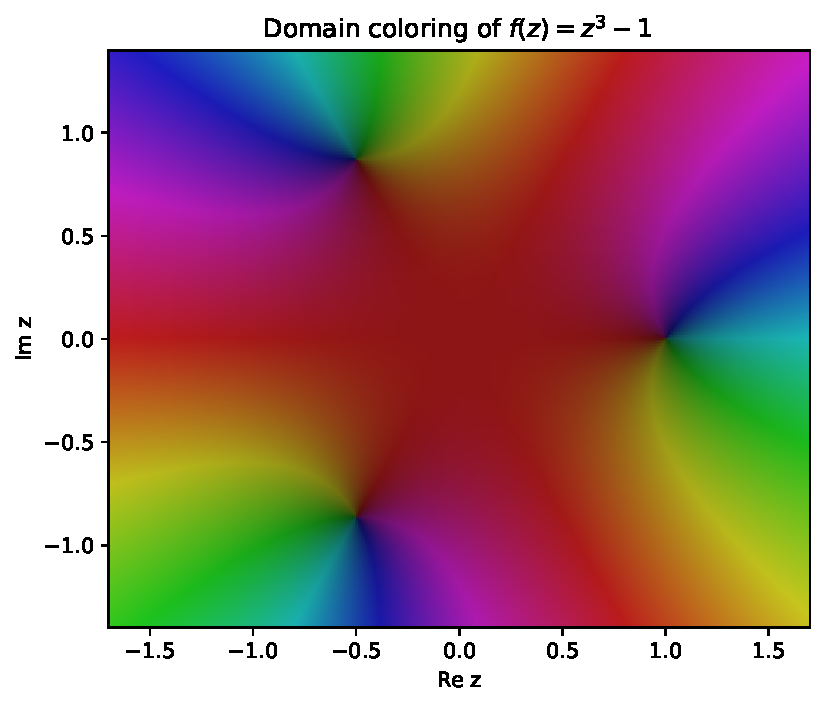
\includegraphics[width=.78\textwidth]{book/parts/part01_mathematical_foundations/chapter05_complex_analysis/figures/generated/domain_coloring.pdf}
\caption{Domain colouring of $f(z)=z^3-1$. The three phase vortices locate the roots of unity.}
\label{fig:ch5-domain-colouring}
\end{figure}

\subsection{Roots of unity}
The script verifies $z_k^n=1$ numerically and plots the regular polygon formed by the roots.

\begin{figure}[htbp]
\centering
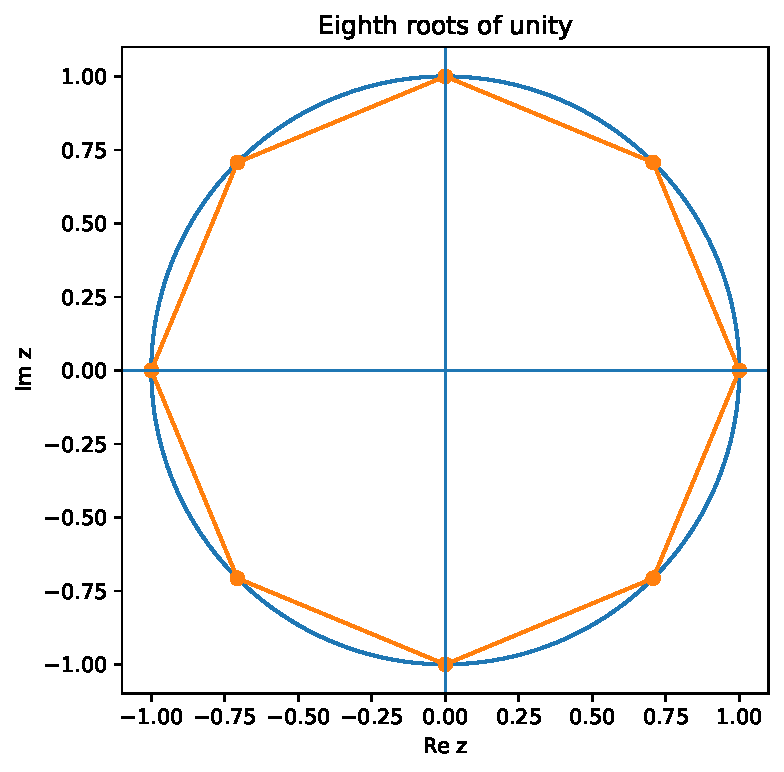
\includegraphics[width=.68\textwidth]{book/parts/part01_mathematical_foundations/chapter05_complex_analysis/figures/generated/roots_of_unity.pdf}
\caption{The eighth roots of unity, equally spaced on the unit circle.}
\label{fig:ch5-roots-computational}
\end{figure}

\subsection{Plane mappings}
A rectangular grid is sampled in the $z$-plane and mapped pointwise under $w=z^2$. The resulting curves make angular doubling and radial squaring visible.

\begin{figure}[htbp]
\centering
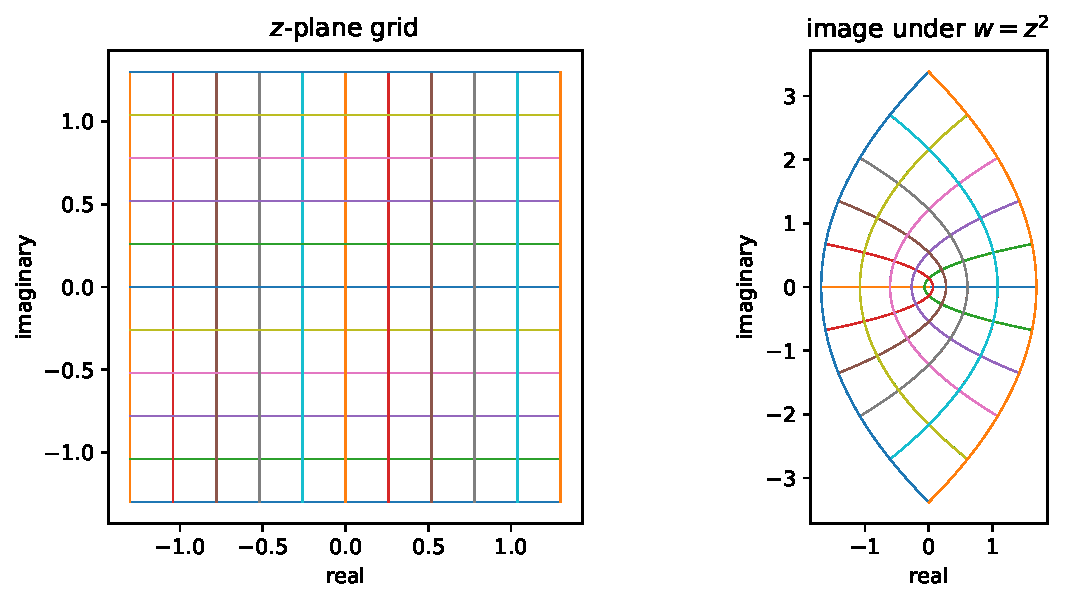
\includegraphics[width=.92\textwidth]{book/parts/part01_mathematical_foundations/chapter05_complex_analysis/figures/generated/square_mapping.pdf}
\caption{A Cartesian grid before and after the map $w=z^2$.}
\label{fig:ch5-square-computational}
\end{figure}

\subsection{Numerical contour integration}
For a parametrized contour $z(t)$, the integral is approximated by a complex trapezoidal rule. Refinement tests confirm
\[
\oint_{|z|=1}\frac{dz}{z}=2\pi i,
\qquad
\oint_{|z|=1}z^3\,dz=0.
\]

\begin{figure}[htbp]
\centering
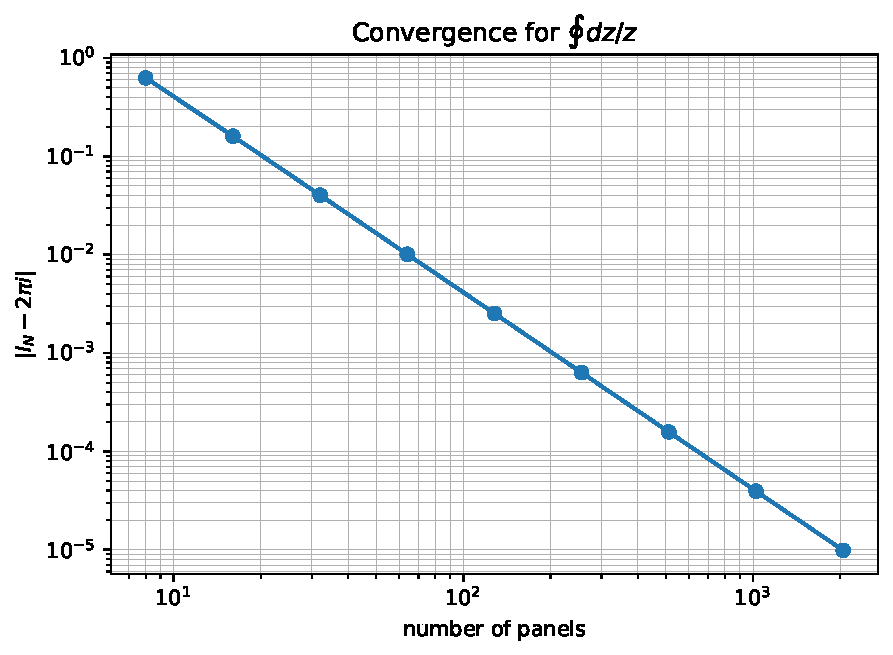
\includegraphics[width=.78\textwidth]{book/parts/part01_mathematical_foundations/chapter05_complex_analysis/figures/generated/contour_convergence.pdf}
\caption{Convergence of the numerical contour integral of $1/z$ around the unit circle.}
\label{fig:ch5-contour-convergence}
\end{figure}

\begin{physicalbox}[Reproducible computation]
Run \texttt{python examples/python/ch05/complex\_analysis\_companion.py}. The program regenerates all four figures, prints root residuals, and reports contour-integral errors. The Wolfram Language file mirrors the symbolic and graphical tasks.
\end{physicalbox}
